 \documentclass[10pt, table, dvipsnames,xcdraw, handout]{beamer}
\usetheme[progressbar=frametitle]{metropolis}
\usepackage{appendixnumberbeamer}
\usetikzlibrary{arrows.meta, positioning, quotes}
\usepackage[shortlabels]{enumitem}
\usepackage{xcolor}
\usepackage{mathtools}


\usepackage{cancel}

\newcommand\hcancel[2][black]{\setbox0=\hbox{$#2$}%
\rlap{\raisebox{.45\ht0}{\textcolor{#1}{\rule{\wd0}{1pt}}}}#2} 


\usepackage{booktabs}
\usepackage[scale=2]{ccicons}

\usepackage{pgfplots}
\usepgfplotslibrary{dateplot}

\usepackage{xspace}
\newcommand{\themename}{\textbf{\textsc{metropolis}}\xspace}
\newcommand{\cb}{\cellcolor{blue!25}}


% Notation:
\newcommand{\cT}{\ensuremath{\mathcal{T}}}
\newcommand{\cD}{\ensuremath{\mathcal{D}}}
\newcommand{\cX}{\ensuremath{\mathcal{X}}}
\newcommand{\cY}{\ensuremath{\mathcal{Y}}}
\newcommand{\cZ}{\ensuremath{\mathcal{Z}}}
\newcommand{\cH}{\ensuremath{\mathcal{H}}}
\newcommand{\cG}{\ensuremath{\mathcal{G}}}

\newcommand{\bR}{\ensuremath{\mathbb{R}}}
\newcommand{\bN}{\ensuremath{\mathbb{N}}}
\newcommand{\bP}{\ensuremath{\mathbb{P}}}
\newcommand{\bT}{\ensuremath{\mathbb{T}}}
\newcommand{\bL}{\ensuremath{\mathbb{L}}}

\newcommand{\bfX}{\ensuremath{\mathbf{X}}}
\newcommand{\bfY}{\ensuremath{\mathbf{Y}}}
\newcommand{\bfy}{\ensuremath{\mathbf{y}}}

\def\layersep{2.5cm}

% Tikz seys
\tikzset{cross/.style={cross out, draw, 
         minimum size=2*(#1-\pgflinewidth), 
         inner sep=0pt, outer sep=0pt}}

\title{Machine Learning I}
\subtitle{Lecture 9: Convolutional Neural Networks}
% \date{\today}
\date{}
\author{Nathaniel Bade}
\institute{Northeastern University Department of Mathematics}
% \titlegraphic{\hfill\includegraphics[height=1.5cm]{logo.pdf}}

\begin{document}

\maketitle

\begin{frame}{Table of contents}
  \setbeamertemplate{section in toc}[sections numbered]
  \tableofcontents[hideallsubsections]
\end{frame}


%%%%%%%%%%%%%% Slidshow Start %%%%%%%%%%%%%% 


\section{Types of Artificial Neural Networks}



\begin{frame}[fragile]{The power of neural networks}
\begin{minipage}[t][0.5\textheight][t]{\textwidth}\centering
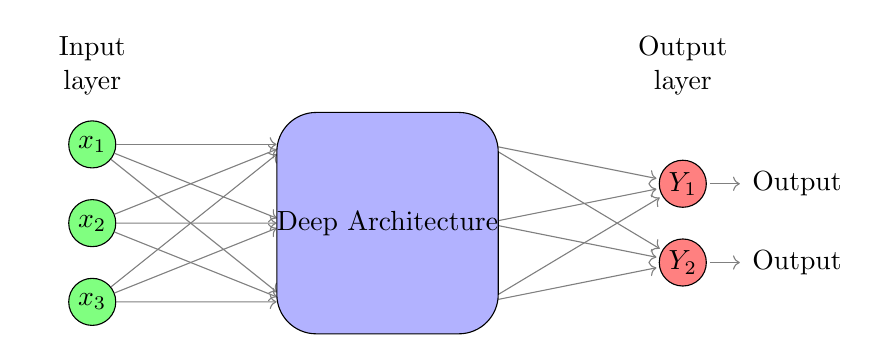
\begin{tikzpicture}[shorten >=1pt,->,draw=black!50, node distance=\layersep]
%https://tex.stackexchange.com/questions/96846/how-to-place-label-in-middle-of-line-above-and-below-with-tikz
    \tikzstyle{every pin edge}=[<-,shorten <=1pt]
    \tikzstyle{neuron}=[circle,fill=black!25,minimum size=17pt,inner sep=0pt, draw=black]
    \tikzstyle{input neuron}=[neuron, fill=green!50];
    \tikzstyle{output neuron}=[neuron, fill=red!50];
    \tikzstyle{hidden neuron}=[neuron, fill=blue!30];
    \tikzstyle{annot} = [text width=4em, text centered]

    % Draw the input layer nodes
    \foreach \name / \y in {1,...,3}
    % This is the same as writing \foreach \name / \y in {1/1,2/2,3/3,4/4}
        \node[input neuron] (I-\name) at (0,-\y) {$x_\y$};

    % Draw the hidden layer nodes
    \foreach \name / \y in {1,...,3}
        \path[yshift=0cm]
            node[] (H1-\name) at (\layersep,-\y cm) {};

    % Draw the hidden layer nodes
    \foreach \name / \y in {1,...,3}
        \path[yshift=0cm]
            node[] (H2-\name) at (\layersep + \layersep,-\y cm) {};


    % Draw the output layer node
    \foreach \name / \y in {1,...,2}
    		\node[output neuron,pin={[pin edge={->}]right:Output}] (O-\y) at (\layersep + \layersep + \layersep,-\y cm-.5cm) {$\,Y_\y\,$};

    % Connect every node in the input layer with every node in the
    % hidden layer.
    \foreach \source in {1,...,3}
        \foreach \dest in {1,...,3}
            \draw (I-\source) --  (H1-\dest);

    % Connect every node in the input layer with every node in the
    % hidden layer.
    \foreach \source in {1,...,3}
        \foreach \dest in {1,...,3}
            \draw (H1-\source) --  (H2-\dest);


    % Connect every node in the hidden layer with the output layer
    \foreach \source in {1,...,3}
		\foreach \dest in {1,...,2}
        		\path (H2-\source) edge (O-\dest);

    % Annotate the layers
    \node[] (H-1) at (\layersep,-1 cm) {};
    
    \node [inner sep=0pt, fill=blue!30, draw=black, outer sep=0pt,minimum size=80pt,rounded corners=0.5cm] (pict1) at (3.75 cm,-2 cm) {Deep Architecture};
    
    \node[annot,above of=H-1, node distance=1cm] (hl) {};
    \node[annot,left of=hl] {Input layer};
    \node[annot,right of=hl] (hl2) {};
    \node[annot,right of=hl2] {Output layer};
    
\end{tikzpicture}
  \end{minipage}
  \vfill
\begin{minipage}[t][0.5\textheight][t]{\textwidth}
Artificial neural networks provide a powerful set of classifiers since for any input shape $\text{dim}(X)$ and any output shape $\text{dim}(Y)$ we have many deep architectures that may allows us to fit the network to the problem at hand. 
\end{minipage}
\end{frame}



\begin{frame}[fragile]{Example: Image Classifier}
\begin{minipage}[t][0.3\textheight][t]{\textwidth}\centering
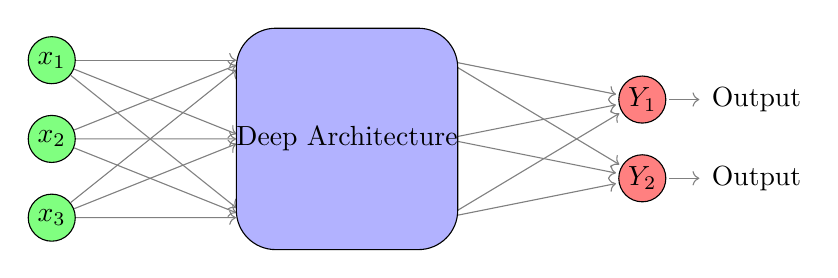
\begin{tikzpicture}[shorten >=1pt,->,draw=black!50, node distance=\layersep]
%https://tex.stackexchange.com/questions/96846/how-to-place-label-in-middle-of-line-above-and-below-with-tikz
    \tikzstyle{every pin edge}=[<-,shorten <=1pt]
    \tikzstyle{neuron}=[circle,fill=black!25,minimum size=17pt,inner sep=0pt, draw=black]
    \tikzstyle{input neuron}=[neuron, fill=green!50];
    \tikzstyle{output neuron}=[neuron, fill=red!50];
    \tikzstyle{hidden neuron}=[neuron, fill=blue!30];
    \tikzstyle{annot} = [text width=4em, text centered]

    % Draw the input layer nodes
    \foreach \name / \y in {1,...,3}
    % This is the same as writing \foreach \name / \y in {1/1,2/2,3/3,4/4}
        \node[input neuron] (I-\name) at (0,-\y) {$x_\y$};

    % Draw the hidden layer nodes
    \foreach \name / \y in {1,...,3}
        \path[yshift=0cm]
            node[] (H1-\name) at (\layersep,-\y cm) {};

    % Draw the hidden layer nodes
    \foreach \name / \y in {1,...,3}
        \path[yshift=0cm]
            node[] (H2-\name) at (\layersep + \layersep,-\y cm) {};


    % Draw the output layer node
    \foreach \name / \y in {1,...,2}
    		\node[output neuron,pin={[pin edge={->}]right:Output}] (O-\y) at (\layersep + \layersep + \layersep,-\y cm-.5cm) {$\,Y_\y\,$};

    % Connect every node in the input layer with every node in the
    % hidden layer.
    \foreach \source in {1,...,3}
        \foreach \dest in {1,...,3}
            \draw (I-\source) --  (H1-\dest);

    % Connect every node in the input layer with every node in the
    % hidden layer.
    \foreach \source in {1,...,3}
        \foreach \dest in {1,...,3}
            \draw (H1-\source) --  (H2-\dest);


    % Connect every node in the hidden layer with the output layer
    \foreach \source in {1,...,3}
		\foreach \dest in {1,...,2}
        		\path (H2-\source) edge (O-\dest);

    % Annotate the layers
    \node[] (H-1) at (\layersep,-1 cm) {};
    
    \node [inner sep=0pt, fill=blue!30, draw=black, outer sep=0pt,minimum size=80pt,rounded corners=0.5cm] (pict1) at (3.75 cm,-2 cm) {Deep Architecture};
    
\end{tikzpicture}
  \end{minipage}
  \vfill
\begin{minipage}[t][0.7\textheight][t]{\textwidth}
Label Classifiers: 
\begin{center}
\includegraphics[height=.3\textheight]{L1DogCat.png}

Input Shape: height $\times$ width. Output Shape: \# Categories.
\end{center}
\end{minipage}
\end{frame}






\begin{frame}[fragile]{Example: Text Classifier}
\begin{minipage}[t][0.3\textheight][t]{\textwidth}\centering
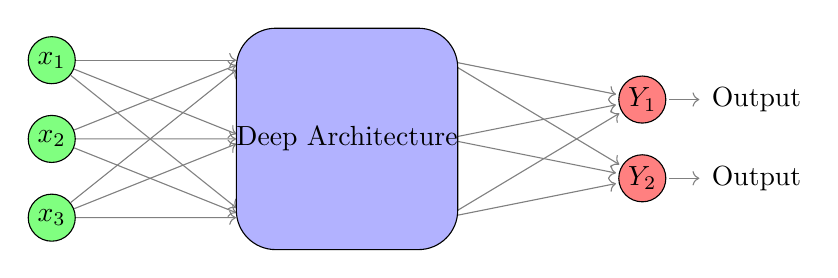
\begin{tikzpicture}[shorten >=1pt,->,draw=black!50, node distance=\layersep]
%https://tex.stackexchange.com/questions/96846/how-to-place-label-in-middle-of-line-above-and-below-with-tikz
    \tikzstyle{every pin edge}=[<-,shorten <=1pt]
    \tikzstyle{neuron}=[circle,fill=black!25,minimum size=17pt,inner sep=0pt, draw=black]
    \tikzstyle{input neuron}=[neuron, fill=green!50];
    \tikzstyle{output neuron}=[neuron, fill=red!50];
    \tikzstyle{hidden neuron}=[neuron, fill=blue!30];
    \tikzstyle{annot} = [text width=4em, text centered]

    % Draw the input layer nodes
    \foreach \name / \y in {1,...,3}
    % This is the same as writing \foreach \name / \y in {1/1,2/2,3/3,4/4}
        \node[input neuron] (I-\name) at (0,-\y) {$x_\y$};

    % Draw the hidden layer nodes
    \foreach \name / \y in {1,...,3}
        \path[yshift=0cm]
            node[] (H1-\name) at (\layersep,-\y cm) {};

    % Draw the hidden layer nodes
    \foreach \name / \y in {1,...,3}
        \path[yshift=0cm]
            node[] (H2-\name) at (\layersep + \layersep,-\y cm) {};


    % Draw the output layer node
    \foreach \name / \y in {1,...,2}
    		\node[output neuron,pin={[pin edge={->}]right:Output}] (O-\y) at (\layersep + \layersep + \layersep,-\y cm-.5cm) {$\,Y_\y\,$};

    % Connect every node in the input layer with every node in the
    % hidden layer.
    \foreach \source in {1,...,3}
        \foreach \dest in {1,...,3}
            \draw (I-\source) --  (H1-\dest);

    % Connect every node in the input layer with every node in the
    % hidden layer.
    \foreach \source in {1,...,3}
        \foreach \dest in {1,...,3}
            \draw (H1-\source) --  (H2-\dest);


    % Connect every node in the hidden layer with the output layer
    \foreach \source in {1,...,3}
		\foreach \dest in {1,...,2}
        		\path (H2-\source) edge (O-\dest);

    % Annotate the layers
    \node[] (H-1) at (\layersep,-1 cm) {};
    
    \node [inner sep=0pt, fill=blue!30, draw=black, outer sep=0pt,minimum size=80pt,rounded corners=0.5cm] (pict1) at (3.75 cm,-2 cm) {Deep Architecture};
    
\end{tikzpicture}
  \end{minipage}
  \vfill
\begin{minipage}[t][0.7\textheight][t]{\textwidth}
Label Classifiers: 
\begin{center}
\includegraphics[width=\textwidth]{realorfake.png}

Input Shape: \#Chars per sting $\times$ \# 26. Output Shape: \# Categories.
\end{center}
\end{minipage}
\end{frame}


\begin{frame}[fragile]{Example: Segmentation}
\begin{minipage}[t][0.3\textheight][t]{\textwidth}\centering
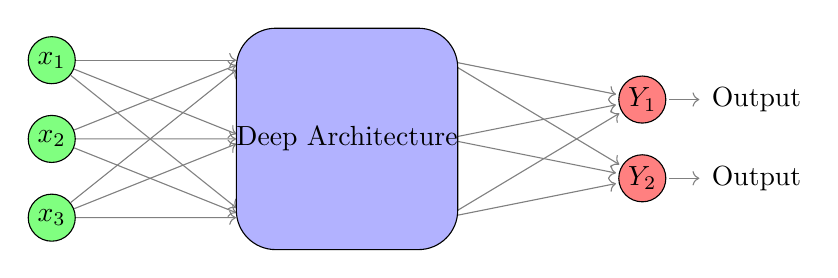
\begin{tikzpicture}[shorten >=1pt,->,draw=black!50, node distance=\layersep]
%https://tex.stackexchange.com/questions/96846/how-to-place-label-in-middle-of-line-above-and-below-with-tikz
    \tikzstyle{every pin edge}=[<-,shorten <=1pt]
    \tikzstyle{neuron}=[circle,fill=black!25,minimum size=17pt,inner sep=0pt, draw=black]
    \tikzstyle{input neuron}=[neuron, fill=green!50];
    \tikzstyle{output neuron}=[neuron, fill=red!50];
    \tikzstyle{hidden neuron}=[neuron, fill=blue!30];
    \tikzstyle{annot} = [text width=4em, text centered]

    % Draw the input layer nodes
    \foreach \name / \y in {1,...,3}
    % This is the same as writing \foreach \name / \y in {1/1,2/2,3/3,4/4}
        \node[input neuron] (I-\name) at (0,-\y) {$x_\y$};

    % Draw the hidden layer nodes
    \foreach \name / \y in {1,...,3}
        \path[yshift=0cm]
            node[] (H1-\name) at (\layersep,-\y cm) {};

    % Draw the hidden layer nodes
    \foreach \name / \y in {1,...,3}
        \path[yshift=0cm]
            node[] (H2-\name) at (\layersep + \layersep,-\y cm) {};


    % Draw the output layer node
    \foreach \name / \y in {1,...,2}
    		\node[output neuron,pin={[pin edge={->}]right:Output}] (O-\y) at (\layersep + \layersep + \layersep,-\y cm-.5cm) {$\,Y_\y\,$};

    % Connect every node in the input layer with every node in the
    % hidden layer.
    \foreach \source in {1,...,3}
        \foreach \dest in {1,...,3}
            \draw (I-\source) --  (H1-\dest);

    % Connect every node in the input layer with every node in the
    % hidden layer.
    \foreach \source in {1,...,3}
        \foreach \dest in {1,...,3}
            \draw (H1-\source) --  (H2-\dest);


    % Connect every node in the hidden layer with the output layer
    \foreach \source in {1,...,3}
		\foreach \dest in {1,...,2}
        		\path (H2-\source) edge (O-\dest);

    % Annotate the layers
    \node[] (H-1) at (\layersep,-1 cm) {};
    
    \node [inner sep=0pt, fill=blue!30, draw=black, outer sep=0pt,minimum size=80pt,rounded corners=0.5cm] (pict1) at (3.75 cm,-2 cm) {Deep Architecture};
    
\end{tikzpicture}
  \end{minipage}
  \vfill
\begin{minipage}[t][0.7\textheight][t]{\textwidth}
Segmentation:
\begin{center}
\includegraphics[height=.3\textheight]{Segmentation.png}

Input Shape: Height $\times$ Width. Output Shape: Height $\times$ Width.
\end{center}
\end{minipage}
\end{frame}






\begin{frame}[fragile]{Example: Object Finder}
\begin{minipage}[t][0.3\textheight][t]{\textwidth}\centering
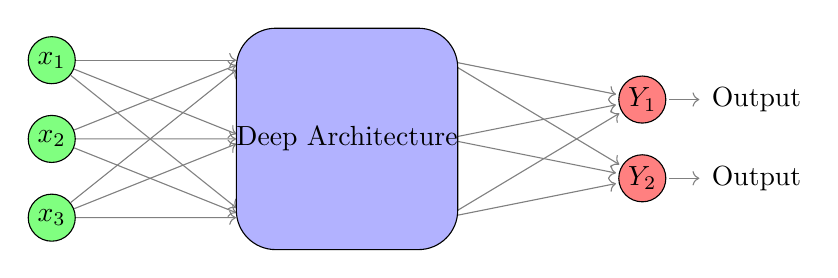
\begin{tikzpicture}[shorten >=1pt,->,draw=black!50, node distance=\layersep]
%https://tex.stackexchange.com/questions/96846/how-to-place-label-in-middle-of-line-above-and-below-with-tikz
    \tikzstyle{every pin edge}=[<-,shorten <=1pt]
    \tikzstyle{neuron}=[circle,fill=black!25,minimum size=17pt,inner sep=0pt, draw=black]
    \tikzstyle{input neuron}=[neuron, fill=green!50];
    \tikzstyle{output neuron}=[neuron, fill=red!50];
    \tikzstyle{hidden neuron}=[neuron, fill=blue!30];
    \tikzstyle{annot} = [text width=4em, text centered]

    % Draw the input layer nodes
    \foreach \name / \y in {1,...,3}
    % This is the same as writing \foreach \name / \y in {1/1,2/2,3/3,4/4}
        \node[input neuron] (I-\name) at (0,-\y) {$x_\y$};

    % Draw the hidden layer nodes
    \foreach \name / \y in {1,...,3}
        \path[yshift=0cm]
            node[] (H1-\name) at (\layersep,-\y cm) {};

    % Draw the hidden layer nodes
    \foreach \name / \y in {1,...,3}
        \path[yshift=0cm]
            node[] (H2-\name) at (\layersep + \layersep,-\y cm) {};


    % Draw the output layer node
    \foreach \name / \y in {1,...,2}
    		\node[output neuron,pin={[pin edge={->}]right:Output}] (O-\y) at (\layersep + \layersep + \layersep,-\y cm-.5cm) {$\,Y_\y\,$};

    % Connect every node in the input layer with every node in the
    % hidden layer.
    \foreach \source in {1,...,3}
        \foreach \dest in {1,...,3}
            \draw (I-\source) --  (H1-\dest);

    % Connect every node in the input layer with every node in the
    % hidden layer.
    \foreach \source in {1,...,3}
        \foreach \dest in {1,...,3}
            \draw (H1-\source) --  (H2-\dest);


    % Connect every node in the hidden layer with the output layer
    \foreach \source in {1,...,3}
		\foreach \dest in {1,...,2}
        		\path (H2-\source) edge (O-\dest);

    % Annotate the layers
    \node[] (H-1) at (\layersep,-1 cm) {};
    
    \node [inner sep=0pt, fill=blue!30, draw=black, outer sep=0pt,minimum size=80pt,rounded corners=0.5cm] (pict1) at (3.75 cm,-2 cm) {Deep Architecture};
    
\end{tikzpicture}
  \end{minipage}
  \vfill
\begin{minipage}[t][0.7\textheight][t]{\textwidth}
Object Finding:
\begin{center}
\includegraphics[height=.3\textheight]{objectfinding.png}

Input Shape: Height $\times$ Width. 

Output Shape: Max \# of Items  $\times$ Box Dims.
\end{center}
\end{minipage}
\end{frame}






\begin{frame}[fragile]{Example: Object Finder}
\begin{minipage}[t][0.3\textheight][t]{\textwidth}\centering
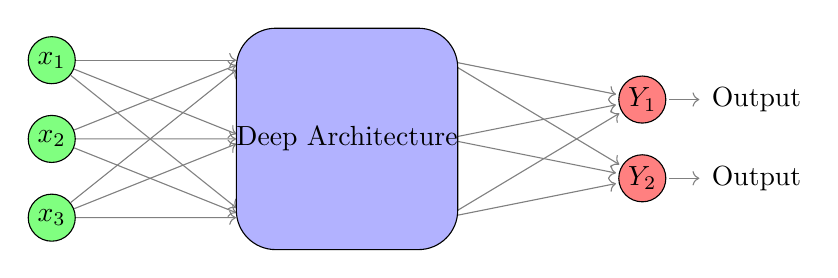
\begin{tikzpicture}[shorten >=1pt,->,draw=black!50, node distance=\layersep]
%https://tex.stackexchange.com/questions/96846/how-to-place-label-in-middle-of-line-above-and-below-with-tikz
    \tikzstyle{every pin edge}=[<-,shorten <=1pt]
    \tikzstyle{neuron}=[circle,fill=black!25,minimum size=17pt,inner sep=0pt, draw=black]
    \tikzstyle{input neuron}=[neuron, fill=green!50];
    \tikzstyle{output neuron}=[neuron, fill=red!50];
    \tikzstyle{hidden neuron}=[neuron, fill=blue!30];
    \tikzstyle{annot} = [text width=4em, text centered]

    % Draw the input layer nodes
    \foreach \name / \y in {1,...,3}
    % This is the same as writing \foreach \name / \y in {1/1,2/2,3/3,4/4}
        \node[input neuron] (I-\name) at (0,-\y) {$x_\y$};

    % Draw the hidden layer nodes
    \foreach \name / \y in {1,...,3}
        \path[yshift=0cm]
            node[] (H1-\name) at (\layersep,-\y cm) {};

    % Draw the hidden layer nodes
    \foreach \name / \y in {1,...,3}
        \path[yshift=0cm]
            node[] (H2-\name) at (\layersep + \layersep,-\y cm) {};


    % Draw the output layer node
    \foreach \name / \y in {1,...,2}
    		\node[output neuron,pin={[pin edge={->}]right:Output}] (O-\y) at (\layersep + \layersep + \layersep,-\y cm-.5cm) {$\,Y_\y\,$};

    % Connect every node in the input layer with every node in the
    % hidden layer.
    \foreach \source in {1,...,3}
        \foreach \dest in {1,...,3}
            \draw (I-\source) --  (H1-\dest);

    % Connect every node in the input layer with every node in the
    % hidden layer.
    \foreach \source in {1,...,3}
        \foreach \dest in {1,...,3}
            \draw (H1-\source) --  (H2-\dest);


    % Connect every node in the hidden layer with the output layer
    \foreach \source in {1,...,3}
		\foreach \dest in {1,...,2}
        		\path (H2-\source) edge (O-\dest);

    % Annotate the layers
    \node[] (H-1) at (\layersep,-1 cm) {};
    
    \node [inner sep=0pt, fill=blue!30, draw=black, outer sep=0pt,minimum size=80pt,rounded corners=0.5cm] (pict1) at (3.75 cm,-2 cm) {Deep Architecture};
    
\end{tikzpicture}
  \end{minipage}
  \vfill
\begin{minipage}[t][0.7\textheight][t]{\textwidth}
Object Generation:
\begin{center}
\includegraphics[height=.3\textheight]{generation.png}

Input Shape: \#Chars per sting $\times$ \# 26. Output Shape: height $\times$ width.
\end{center}
\end{minipage}
\end{frame}









\begin{frame}[fragile]{Example: Object Finder}
\begin{minipage}[t][0.3\textheight][t]{\textwidth}\centering
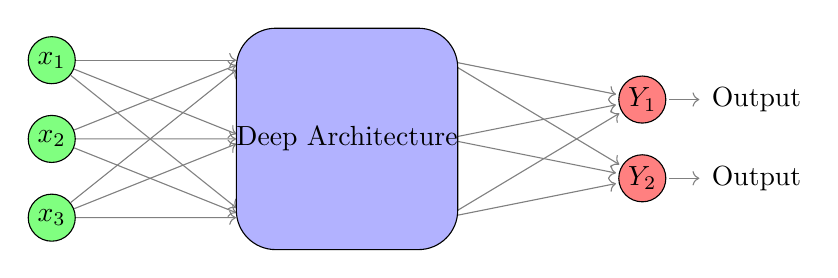
\begin{tikzpicture}[shorten >=1pt,->,draw=black!50, node distance=\layersep]
%https://tex.stackexchange.com/questions/96846/how-to-place-label-in-middle-of-line-above-and-below-with-tikz
    \tikzstyle{every pin edge}=[<-,shorten <=1pt]
    \tikzstyle{neuron}=[circle,fill=black!25,minimum size=17pt,inner sep=0pt, draw=black]
    \tikzstyle{input neuron}=[neuron, fill=green!50];
    \tikzstyle{output neuron}=[neuron, fill=red!50];
    \tikzstyle{hidden neuron}=[neuron, fill=blue!30];
    \tikzstyle{annot} = [text width=4em, text centered]

    % Draw the input layer nodes
    \foreach \name / \y in {1,...,3}
    % This is the same as writing \foreach \name / \y in {1/1,2/2,3/3,4/4}
        \node[input neuron] (I-\name) at (0,-\y) {$x_\y$};

    % Draw the hidden layer nodes
    \foreach \name / \y in {1,...,3}
        \path[yshift=0cm]
            node[] (H1-\name) at (\layersep,-\y cm) {};

    % Draw the hidden layer nodes
    \foreach \name / \y in {1,...,3}
        \path[yshift=0cm]
            node[] (H2-\name) at (\layersep + \layersep,-\y cm) {};


    % Draw the output layer node
    \foreach \name / \y in {1,...,2}
    		\node[output neuron,pin={[pin edge={->}]right:Output}] (O-\y) at (\layersep + \layersep + \layersep,-\y cm-.5cm) {$\,Y_\y\,$};

    % Connect every node in the input layer with every node in the
    % hidden layer.
    \foreach \source in {1,...,3}
        \foreach \dest in {1,...,3}
            \draw (I-\source) --  (H1-\dest);

    % Connect every node in the input layer with every node in the
    % hidden layer.
    \foreach \source in {1,...,3}
        \foreach \dest in {1,...,3}
            \draw (H1-\source) --  (H2-\dest);


    % Connect every node in the hidden layer with the output layer
    \foreach \source in {1,...,3}
		\foreach \dest in {1,...,2}
        		\path (H2-\source) edge (O-\dest);

    % Annotate the layers
    \node[] (H-1) at (\layersep,-1 cm) {};
    
    \node [inner sep=0pt, fill=blue!30, draw=black, outer sep=0pt,minimum size=80pt,rounded corners=0.5cm] (pict1) at (3.75 cm,-2 cm) {Deep Architecture};
    
\end{tikzpicture}
  \end{minipage}
  \vfill
\begin{minipage}[t][0.7\textheight][t]{\textwidth}
The challenge of course is filling in the middle for each of these cases, while taking into consideration training time, data composition and computational power. The appeal of neural networks is that it's very easy to set a problem up computational power alone will solve it. 

Sometimes, this is the case as with the MNIST data set and the perceptron networks. But often a clever solution requires more complex architecture than just densely connected layers. 
\end{minipage}
\end{frame}




\begin{frame}[fragile]{Genre of Artificial Neural Networks}
Modern artificial neural networks can be sorted into three broad categories based on their structure:

\begin{itemize}
\item[] Feed forward networks: A trained feed forward network acts like a function, taking in a set of data at one end and returning a new set of data at the other.\pause

\item[] Recurrent networks: Trained recurrent networks are stateful. That is, RNN's take data and return an output but the remember the last $M$ pieces of data sent through in an internal \textbf{state}. \pause

\item[] Symmetrically Connected Networks: A trained SCN is a densely connected network with an update rule. For any initial value of the nodes, the function ``updates," moving at each step towards a ``lower energy state". The result is achieved when updating no longer changes the sate. 
\end{itemize}
\end{frame}





\begin{frame}[fragile]{Feed Forward Networks}
  \begin{minipage}[t][0.5\textheight][t]{\textwidth}
	\centering \includegraphics[height=0.5\textheight]{L12FFNetwork.png} 
  \end{minipage}
  \vfill
\begin{minipage}[t][0.5\textheight][t]{\textwidth}
Feed forward networks are the most common type, they take an input, process it through a series of operation, and return some output. \newline\pause 

Mathematically they are just functions $f_\beta (X)$ depending on some trainable parameters $\beta$. They could result in a classifier $\hat{y} = f_\beta (X)$, or a loss function $\ell(X,z) = f_\beta (X)$. 
\end{minipage}
\end{frame}





\begin{frame}[fragile]{Feed Forward Networks}
  \begin{minipage}[t][0.5\textheight][t]{\textwidth}
	\centering \includegraphics[height=0.5\textheight]{L12Deconv.png} 
  \end{minipage}
  \vfill
\begin{minipage}[t][0.5\textheight][t]{\textwidth}
For example feed forward networks can be labeling or regression, but they can also be generative networks (returning more data) or unsupervised, returning a dimensional reduction, clustering or other description of the data. \newline \pause

However, once trained the weights $\beta$ are \textbf{fixed} for all prediction.
\end{minipage}
\end{frame}



\begin{frame}[fragile]{Recurrent Networks}
  \begin{minipage}[t][0.5\textheight][t]{\textwidth}
	\centering \includegraphics[height=0.5\textheight]{L12RNN.png} 
  \end{minipage}
  \vfill
\begin{minipage}[t][0.5\textheight][t]{\textwidth}
A recurrent neural network has state variables that can be changed at runtime and that persist between prediction runs.\pause\newline

For example, in text prediction an RNN may predict one word at a time while "remembering" its previous predictions. 
\end{minipage}
\end{frame}



\begin{frame}[fragile]{Recurrent Networks}
  \begin{minipage}[t][0.5\textheight][t]{\textwidth}
	\centering \includegraphics[height=0.5\textheight]{L12RNN2.png} 
  \end{minipage}
  \vfill
\begin{minipage}[t][0.5\textheight][t]{\textwidth}
A recurrent neural network on the other hand has state variables that can be changed at runtime and that persist between prediction runs.\newline

For example, in text prediction an RNN may predict one word at a time while "remembering" its previous predictions. 
\end{minipage}
\end{frame}




\begin{frame}[fragile]{Recurrent Networks}
  \begin{minipage}[t][0.5\textheight][t]{\textwidth}
	\centering \includegraphics[height=0.5\textheight]{L12RNN3.png} 
  \end{minipage}
  \vfill
\begin{minipage}[t][0.5\textheight][t]{\textwidth}
A recurrent node is often represented in ``wrapped" form as above. RNN's are used extensively in time series prediction and natural language processing, although there success is still under scrutiny. 
\end{minipage}
\end{frame}





\begin{frame}[fragile]{Types of Feed Forward Networks}
The following are a list of common network types and their uses

\begin{itemize}
\item[] \textbf{Multilayer perceptron networks} - Stacks of almost linear classifiers for labeling. \pause
\item[] \textbf{Radial basis function networks} - Perceptron algorithms tweaked to find cluster centers.  \pause
\item[] \textbf{Convolutional Networks} - Spatially aware classifiers.\pause
\item[] \textbf{Autoencoders} - Dimensional reduction networks. \pause
\item[] \textbf{Generative adversarial network} - Example generation networks. \pause
\end{itemize}
Fjodor Van Veen has compiled a zoo of common architectures: 
\url{https://www.asimovinstitute.org/author/fjodorvanveen/}
\end{frame}


\begin{frame}[fragile]{Summary}
We will now go into the details of convolutional neural networks. Convolutional networks differ from perceptrons by building spacial reasoning directly into their architecture. \newline\pause

In the third part of the lecture, we will discuss \textbf{long term short term} (\textbf{LSTM}) networks as examples of recurrent networks. Both of these architectures are implemented in Tensorflow and Keras, and are still not completely understood mathematically. \pause\newline

Almost all modern networks are built out variations of perceptrons, CNNs and RNNs.
\end{frame}



\section{Convolutional Neural Networks}



\begin{frame}[fragile]{CNN}
  \begin{minipage}[t][0.5\textheight][t]{\textwidth}
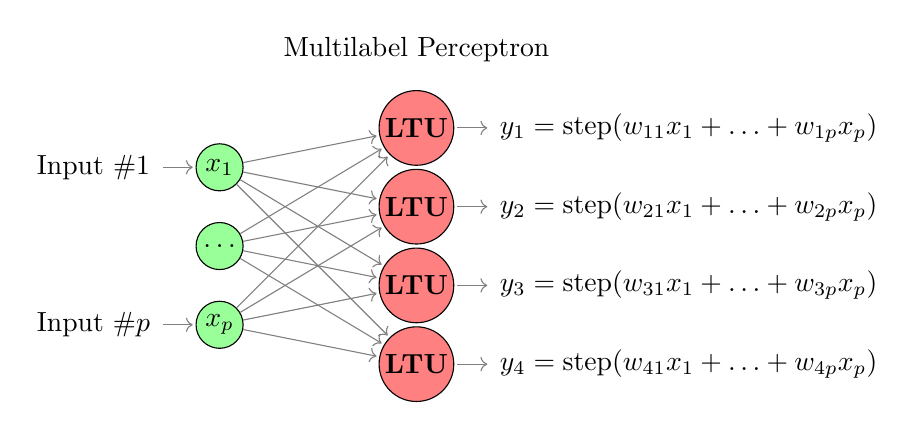
\begin{tikzpicture}[shorten >=1pt,->,draw=black!50, node distance=\layersep]
%https://tex.stackexchange.com/questions/96846/how-to-place-label-in-middle-of-line-above-and-below-with-tikz
    \tikzstyle{every pin edge}=[<-,shorten <=1pt]
    \tikzstyle{neuron}=[circle,fill=black!25,minimum size=17pt,inner sep=0pt, draw=black]
    \tikzstyle{input neuron}=[neuron, fill=green!40];
    \tikzstyle{output neuron}=[neuron, fill=red!50];
    \tikzstyle{hidden neuron}=[neuron, fill=blue!30];
    \tikzstyle{annot} = [text width=10em, text centered]

    % Draw the input layer nodes
	\node[input neuron, pin=left:Input \#1] (I-1) at (0,-1) {$x_1$};
	\node[input neuron] (I-2) at (0,-2) {$\ldots$};
	\node[input neuron, pin=left:Input \#$p$] (I-3) at (0,-3) {$x_p$};
        

    % Draw the hidden layer nodes
	\foreach \name / \y in {1,...,4}
        \node[output neuron, pin={[pin edge={->}]right: $y_\y=\text{step}(w_{\y 1}x_1+\ldots+ w_{\y p}x_p)$ }] (H-\y) at (\layersep,.5cm - \y cm) {$\,\textbf{LTU}\,$};

    \foreach \source in {1,...,3}
        \foreach \dest in {1,...,4}
		  \draw (I-\source) -- (H-\dest);


    \node[annot,above of=H-1, node distance=1cm] (hl) {Multilabel Perceptron};
\end{tikzpicture}
  \end{minipage}
  \vfill
\begin{minipage}[t][0.5\textheight][t]{\textwidth}
Recall that the multilayer perceptron treats all of it's input variables as being on exactly equal footing. During training, the weights will be reconfigured to preference certain combinations of inputs over others. \pause Any structure between the input features must be discovered by the network. 
\end{minipage}
\end{frame}





\begin{frame}[fragile]{CNN}
  \begin{minipage}[t][0.5\textheight][t]{\textwidth}\centering
\begin{tikzpicture}[shorten >=1pt,->,draw=black!50, node distance=\layersep]
%https://tex.stackexchange.com/questions/96846/how-to-place-label-in-middle-of-line-above-and-below-with-tikz
    \tikzstyle{every pin edge}=[<-,shorten <=1pt]
    \tikzstyle{neuron}=[circle,fill=black!25,minimum size=17pt,inner sep=0pt, draw=black]
    \tikzstyle{input neuron}=[neuron, fill=green!40];
    \tikzstyle{output neuron}=[neuron, fill=red!50];
    \tikzstyle{hidden neuron}=[neuron, fill=blue!30];
    \tikzstyle{annot} = [text width=10em, text centered]

	\node[inner sep=0pt] (pic) at (-4,-2){\includegraphics[width=.2\textwidth]{L12PIC.png}};
	\node[inner sep=0pt] (upic) at (-1.5,-2){\includegraphics[height=.5\textheight]{L12PIC2.png}};

    % Draw the input layer nodes
	\node[input neuron] (I-1) at (0,-1) {$x_1$};
	\node[input neuron] (I-2) at (0,-2) {$\ldots$};
	\node[input neuron] (I-3) at (0,-3) {$x_p$};
        

    % Draw the hidden layer nodes
	\foreach \name / \y in {1,...,4}
        \node[output neuron] (H-\y) at (\layersep,.5cm - \y cm) {$\,\textbf{LTU}\,$};

    \foreach \source in {1,...,3}
        \foreach \dest in {1,...,4}
		  \draw (I-\source) -- (H-\dest);

	\draw (pic) -- (upic);
	\draw (upic.north east) -- (I-1);
	\draw (upic) -- (I-2);
	\draw (upic.south east) -- (I-3);

    \node[annot,above of=H-1, node distance=1cm] (hl) {Multilabel Perceptron};
\end{tikzpicture}
  \end{minipage}
  \vfill
\begin{minipage}[t][0.5\textheight][t]{\textwidth}
For example, when processing a picture the first step is to unspool the 2d image into a 1d vector. \pause This forgets about the spacial nature of the training data. 
\end{minipage}
\end{frame}




\begin{frame}[fragile]{CNN}
  \begin{minipage}[t][0.5\textheight][t]{\textwidth}\centering
\begin{tikzpicture}[shorten >=1pt,->,draw=black!50, node distance=\layersep]
%https://tex.stackexchange.com/questions/96846/how-to-place-label-in-middle-of-line-above-and-below-with-tikz
    \tikzstyle{every pin edge}=[<-,shorten <=1pt]
    \tikzstyle{neuron}=[circle,fill=black!25,minimum size=17pt,inner sep=0pt, draw=black]
    \tikzstyle{input neuron}=[neuron, fill=green!40];
    \tikzstyle{output neuron}=[neuron, fill=red!50];
    \tikzstyle{hidden neuron}=[neuron, fill=blue!30];
    \tikzstyle{annot} = [text width=10em, text centered]

	\node[inner sep=0pt] (pic) at (-4,-2){\includegraphics[width=.2\textwidth]{L12PIC.png}};
	\node[inner sep=0pt] (upic) at (-1.5,-2){\includegraphics[height=.5\textheight]{L12PIC2.png}};

    % Draw the input layer nodes
	\node[input neuron] (I-1) at (0,-1) {$x_1$};
	\node[input neuron] (I-2) at (0,-2) {$\ldots$};
	\node[input neuron] (I-3) at (0,-3) {$x_p$};
        

    % Draw the hidden layer nodes
	\foreach \name / \y in {1,...,4}
        \node[output neuron] (H-\y) at (\layersep,.5cm - \y cm) {$\,\textbf{LTU}\,$};

    \foreach \source in {1,...,3}
        \foreach \dest in {1,...,4}
		  \draw (I-\source) -- (H-\dest);

	\draw (pic) -- (upic);
	\draw (upic.north east) -- (I-1);
	\draw (upic) -- (I-2);
	\draw (upic.south east) -- (I-3);

    \node[annot,above of=H-1, node distance=1cm] (hl) {Multilabel Perceptron};
\end{tikzpicture}
  \end{minipage}
  \vfill
\begin{minipage}[t][0.5\textheight][t]{\textwidth}
This has two huge problems: 

1) The network has to ``learn'' which nodes are next to each other, and thus should be correlated. 

\end{minipage}
\end{frame}


\begin{frame}[fragile]{CNN}
  \begin{minipage}[t][0.5\textheight][t]{\textwidth}\centering
\begin{tikzpicture}[shorten >=1pt,->,draw=black!50, node distance=\layersep]
%https://tex.stackexchange.com/questions/96846/how-to-place-label-in-middle-of-line-above-and-below-with-tikz
    \tikzstyle{every pin edge}=[<-,shorten <=1pt]
    \tikzstyle{neuron}=[circle,fill=black!25,minimum size=17pt,inner sep=0pt, draw=black]
    \tikzstyle{input neuron}=[neuron, fill=green!40];
    \tikzstyle{output neuron}=[neuron, fill=red!50];
    \tikzstyle{hidden neuron}=[neuron, fill=blue!30];
    \tikzstyle{annot} = [text width=10em, text centered]

	\node[inner sep=0pt] (pic) at (-4,-2){\includegraphics[width=.2\textwidth]{L12PIC.png}};
	\node[inner sep=0pt] (upic) at (-1.5,-2){\includegraphics[height=.5\textheight]{L12PIC2.png}};

    % Draw the input layer nodes
	\node[input neuron] (I-1) at (0,-1) {$x_1$};
	\node[input neuron] (I-2) at (0,-2) {$\ldots$};
	\node[input neuron] (I-3) at (0,-3) {$x_p$};
        

    % Draw the hidden layer nodes
	\foreach \name / \y in {1,...,4}
        \node[output neuron] (H-\y) at (\layersep,.5cm - \y cm) {$\,\textbf{LTU}\,$};

    \foreach \source in {1,...,3}
        \foreach \dest in {1,...,4}
		  \draw (I-\source) -- (H-\dest);

	\draw (pic) -- (upic);
	\draw (upic.north east) -- (I-1);
	\draw (upic) -- (I-2);
	\draw (upic.south east) -- (I-3);

    \node[annot,above of=H-1, node distance=1cm] (hl) {Multilabel Perceptron};
\end{tikzpicture}
  \end{minipage}
  \vfill
\begin{minipage}[t][0.5\textheight][t]{\textwidth}
This has two huge problems: 

2) Features discovered are \emph{not translation invariant}. This may be fine for the MNIST dataset where all of the features are centered and very distinct, but on a more complicated dataset we must learn our features \emph{for every possible translation}.
\end{minipage}
\end{frame}


\begin{frame}[fragile]{CNN}
  \begin{minipage}[t][0.5\textheight][t]{\textwidth}\centering
\begin{center}
\includegraphics[height=.5\textheight]{LocalNN.png}
\end{center}
  \end{minipage}
  \vfill
\begin{minipage}[t][0.5\textheight][t]{\textwidth}
We want to construct a network that has spacial locality and translation invariance built in from the start. One simple way to enforce locality is to just kill off all non-local connections between node. Practically, this means we put in a single node for each $n\times n$ sub-rectangle of points. For an $H\times W$ image, this means we will have
$$
\text{\# Hidden Nodes:}\,\,\, (H-n)\times (W-n)
$$
\end{minipage}
\end{frame}



\begin{frame}[fragile]{CNN}
  \begin{minipage}[t][0.5\textheight][t]{\textwidth}\centering
\begin{center}
\includegraphics[height=.5\textheight]{LocalNN2.png}
\end{center}
  \end{minipage}
  \vfill
\begin{minipage}[t][0.5\textheight][t]{\textwidth}
These of course can then be fed into a more layers for further classification. 
\end{minipage}
\end{frame}




\begin{frame}[fragile]{CNN}
  \begin{minipage}[t][0.5\textheight][t]{\textwidth}\centering
\begin{center}
\includegraphics[height=.5\textheight]{LocalNN.png}
\end{center}
  \end{minipage}
  \vfill
\begin{minipage}[t][0.5\textheight][t]{\textwidth}
This solves the locality problem, but doesn't really solve translation invariance. Each node in the first hidden layer will eventually optimize to finding a single set of features for each $n\times n$ square, but 

\begin{itemize}
\item{1)}Features learned at one position won't translate to feature learned at another. 
\item{2)} We may want to learn more than one set of features at each location. 
\end{itemize}
\end{minipage}
\end{frame}

\begin{frame}[fragile]{CNN}
  \begin{minipage}[t][0.5\textheight][t]{\textwidth}\centering
\begin{center}
\includegraphics[height=.5\textheight]{LocalNN3.png}
\end{center}
  \end{minipage}
  \vfill
\begin{minipage}[t][0.5\textheight][t]{\textwidth}
What we really want is to fit a set $F$ of feature \emph{simultaneously} to each $n\times n$ rectangle. In ANN language, we want each $n\times n$ rectangle to attach to $F$ distinct nodes. Each node can then specialize it's weights to detecting exactly one feature, and all of these features can be filtered into the the dense layers. 
\end{minipage}
\end{frame}



\begin{frame}[fragile]{CNN}
  \begin{minipage}[t][0.5\textheight][t]{\textwidth}\centering
\begin{center}
\includegraphics[height=.5\textheight]{LocalNN4.png}
\end{center}
  \end{minipage}
  \vfill
\begin{minipage}[t][0.5\textheight][t]{\textwidth}
Finally, to make the fit simultaneous, we stipulate that the weights for each of the $F$ features for each $n\times n$ box are actually the \emph{same}. This allows us to train all of our network features simultaneous, and truly implements translation invarience. It also drastically lowers the number of number of weights in our network, allowing for quicker training (although we have to think a bit about how to implement back-propagation).
\end{minipage}
\end{frame}




\begin{frame}[fragile]{CNN}
  \begin{minipage}[t][0.5\textheight][t]{\textwidth}\centering
\begin{center}
\includegraphics[height=.5\textheight]{LocalNN4.png}
\end{center}
  \end{minipage}
  \vfill
\begin{minipage}[t][0.5\textheight][t]{\textwidth}
Such a network is called a \textbf{Convolutional Neural Network} because each of the nodes in performing a convolution. For square data with pixel matrix $X_{st}$, the $f$'th feature node value is found by computing
$$
\textbf{Conv Node: } N_{ab}^f = \sigma\left(\sum_{i = 1}^n\sum_{j=1}^n  W_{i,j}^fX_{a+i, b+j} \right)
$$
\end{minipage}
\end{frame}












\begin{frame}[fragile]{Convolutions}
  \begin{minipage}[t][0.5\textheight][t]{\textwidth}\centering
	\centering \includegraphics[height=0.5\textheight]{L12Conv1.png} 
  \end{minipage}
  \vfill
\begin{minipage}[t][0.5\textheight][t]{\textwidth}
Mathematically, a convolution combines two matrices to make a third, by taking the dot product of the smaller matrix with every block of the larger. \pause Formally, for a $m\times n$ matrix $K$ and a $(i+m)\times (j+n)$ matrix $K$, the convolution matrix is
$$
(I*K)_{i,j} = \sum_{s=0}^{m-1}\sum_{r=0}^{n-1} I_{i+s,j+r}K_{s,r}
$$
\end{minipage}
\end{frame}




\begin{frame}[fragile]{Convolutions}
  \begin{minipage}[t][0.5\textheight][t]{\textwidth}\centering
\begin{tikzpicture}[shorten >=1pt,->,draw=black!50, node distance=\layersep]
%https://tex.stackexchange.com/questions/96846/how-to-place-label-in-middle-of-line-above-and-below-with-tikz
    \tikzstyle{every pin edge}=[<-,shorten <=1pt]
    \tikzstyle{neuron}=[circle,fill=black!25,minimum size=17pt,inner sep=0pt, draw=black]
    \tikzstyle{input neuron}=[neuron, fill=green!40];
    \tikzstyle{output neuron}=[neuron, fill=red!50];
    \tikzstyle{hidden neuron}=[neuron, fill=blue!30];
    \tikzstyle{annot} = [text width=10em, text centered]

	\node[inner sep=0pt] (pic) at (-4,-2){\includegraphics[width=.2\textwidth]{L12ConvOrg.png}};
	\node[inner sep=0pt]  at (-2.5,-2){*};
	\node[inner sep=0pt] (conv) at (-1,-2){\includegraphics[width=.2\textwidth]{L12ConvMat.png}};
	\node[inner sep=0pt] (cimg) at (2,-2){\includegraphics[width=.2\textwidth]{L12ConvOrg2.png}};

	\draw (conv) -- (cimg);


    \node[annot] (-1,0) {Edge Detection};
\end{tikzpicture}
  \end{minipage}
  \vfill
\begin{minipage}[t][0.5\textheight][t]{\textwidth}
In image processing, this is used to create effects and extract information from images, including 

\begin{itemize}
\item[] Finding edges 
\end{itemize}
\end{minipage}
\end{frame}



\begin{frame}[fragile]{Convolutions}
  \begin{minipage}[t][0.5\textheight][t]{\textwidth}\centering
\begin{tikzpicture}[shorten >=1pt,->,draw=black!50, node distance=\layersep]
%https://tex.stackexchange.com/questions/96846/how-to-place-label-in-middle-of-line-above-and-below-with-tikz
    \tikzstyle{every pin edge}=[<-,shorten <=1pt]
    \tikzstyle{neuron}=[circle,fill=black!25,minimum size=17pt,inner sep=0pt, draw=black]
    \tikzstyle{input neuron}=[neuron, fill=green!40];
    \tikzstyle{output neuron}=[neuron, fill=red!50];
    \tikzstyle{hidden neuron}=[neuron, fill=blue!30];
    \tikzstyle{annot} = [text width=10em, text centered]

	\node[inner sep=0pt] (pic) at (-4,-2){\includegraphics[width=.2\textwidth]{L12ConvOrg.png}};
	\node[inner sep=0pt]  at (-2.5,-2){*};
	\node[inner sep=0pt] (conv) at (-1,-2){\includegraphics[width=.2\textwidth]{L12ConvMat2.png}};
	\node[inner sep=0pt] (cimg) at (2,-2){\includegraphics[width=.2\textwidth]{L12ConvOrg4.png}};

	\draw (conv) -- (cimg);


    \node[annot] (-1,0) {Edge Detection};
\end{tikzpicture}
  \end{minipage}
  \vfill
\begin{minipage}[t][0.5\textheight][t]{\textwidth}
In image processing, this is used to create effects and extract information from images, including
\begin{itemize}
\item[] Finding edges 
\item[] Blurring
\end{itemize}
\end{minipage}
\end{frame}



\begin{frame}[fragile]{Convolutions}
  \begin{minipage}[t][0.5\textheight][t]{\textwidth}\centering
\begin{tikzpicture}[shorten >=1pt,->,draw=black!50, node distance=\layersep]
%https://tex.stackexchange.com/questions/96846/how-to-place-label-in-middle-of-line-above-and-below-with-tikz
    \tikzstyle{every pin edge}=[<-,shorten <=1pt]
    \tikzstyle{neuron}=[circle,fill=black!25,minimum size=17pt,inner sep=0pt, draw=black]
    \tikzstyle{input neuron}=[neuron, fill=green!40];
    \tikzstyle{output neuron}=[neuron, fill=red!50];
    \tikzstyle{hidden neuron}=[neuron, fill=blue!30];
    \tikzstyle{annot} = [text width=10em, text centered]

	\node[inner sep=0pt] (pic) at (-4,-2){\includegraphics[width=.2\textwidth]{L12ConvOrg.png}};
	\node[inner sep=0pt]  at (-2.5,-2){*};
	\node[inner sep=0pt] (conv) at (-1,-2){\includegraphics[width=.2\textwidth]{L12ConvMat3.png}};
	\node[inner sep=0pt] (cimg) at (2,-2){\includegraphics[width=.2\textwidth]{L12ConvOrg3.png}};

	\draw (conv) -- (cimg);


    \node[annot] (-1,0) {Edge Detection};
\end{tikzpicture}
  \end{minipage}
  \vfill
\begin{minipage}[t][0.5\textheight][t]{\textwidth}
In image processing, this is used to create effects and extract information from images, including
\begin{itemize}
\item[] Finding edges 
\item[] Blurring
\item[] Sharpening
\end{itemize}
\end{minipage}
\end{frame}







\begin{frame}[fragile]{Convolution In Neural Networks}
  \begin{minipage}[t][0.5\textheight][t]{\textwidth}\centering
	\centering \includegraphics[height=0.5\textheight]{L12CNNs.png} 
  \end{minipage}
  \vfill
\begin{minipage}[t][0.5\textheight][t]{\textwidth}
In the world of \textbf{convolutional neural networks}, the convolution matrices play a slightly different role, giving patterns that detect features emblematic of the classification. 
\end{minipage}
\end{frame}




\begin{frame}[fragile]{Convolution In Neural Networks}
  \begin{minipage}[t][0.5\textheight][t]{\textwidth}\centering
	\centering \includegraphics[height=0.5\textheight]{L12ConvLayer.png} 
  \end{minipage}
  \vfill
\begin{minipage}[t][0.5\textheight][t]{\textwidth}
Of course, we are interested in many features so at each convolution step in operation tree we perform $m$ convolutions with weight matrices $W_i$. \pause For each convolution we fit a matrix of weights 
$$
W_i = \left(\begin{matrix}
w^{(i)}_{11}&\ldots&w^{(i)}_{1k}
\\
\vdots &\ddots&\vdots
\\
w^{(i)}_{j1}&\ldots&w^{(i)}_{jk}
\end{matrix}\right)
$$
\end{minipage}
\end{frame}






\begin{frame}[fragile]{Pooling Layers}
  \begin{minipage}[t][0.5\textheight][t]{\textwidth}\centering
\begin{tikzpicture}[shorten >=1pt,->,draw=black!50, node distance=\layersep]
%https://tex.stackexchange.com/questions/96846/how-to-place-label-in-middle-of-line-above-and-below-with-tikz
    \tikzstyle{every pin edge}=[<-,shorten <=1pt]
    \tikzstyle{neuron}=[circle,fill=black!25,minimum size=17pt,inner sep=0pt, draw=black]
    \tikzstyle{input neuron}=[neuron, fill=green!40];
    \tikzstyle{output neuron}=[neuron, fill=red!50];
    \tikzstyle{hidden neuron}=[neuron, fill=blue!30];
    \tikzstyle{annot} = [text width=10em, text centered]

	\node[inner sep=0pt] (pic) at (-2,-2){\includegraphics[width=.3\textwidth]{L12MaxPool.png}};
	\node[inner sep=0pt] (mp) at (2,-2){\includegraphics[width=.2\textwidth]{L12MaxPool2.png}};

	\draw (pic.north east) -- (mp.north west);
	\draw (pic.east) -- (mp.west);
	\draw (pic.south east) -- (mp.south west);



    \node[annot] (1,0) {Max Pooling};
\end{tikzpicture}
  \end{minipage}
  \vfill
\begin{minipage}[t][0.5\textheight][t]{\textwidth}
Successive convolution layers will find higher order features (collections of lower order features) but to group them efficiently it's common to start including pooling layers. A pooling layer down samples an image by taking the max, average, or min of a $n\times m$ set of pixels. 
\end{minipage}
\end{frame}






\begin{frame}[fragile]{Pooling Layers}
  \begin{minipage}[t][0.5\textheight][t]{\textwidth}\centering
\begin{tikzpicture}[shorten >=1pt,->,draw=black!50, node distance=\layersep]
%https://tex.stackexchange.com/questions/96846/how-to-place-label-in-middle-of-line-above-and-below-with-tikz
    \tikzstyle{every pin edge}=[<-,shorten <=1pt]
    \tikzstyle{neuron}=[circle,fill=black!25,minimum size=17pt,inner sep=0pt, draw=black]
    \tikzstyle{input neuron}=[neuron, fill=green!40];
    \tikzstyle{output neuron}=[neuron, fill=red!50];
    \tikzstyle{hidden neuron}=[neuron, fill=blue!30];
    \tikzstyle{annot} = [text width=10em, text centered]

	\node[inner sep=0pt] (pic) at (-2,-2){\includegraphics[width=.3\textwidth]{L12MaxPool.png}};
	\node[inner sep=0pt] (mp) at (2,-2){\includegraphics[width=.2\textwidth]{L12MaxPool3.png}};

	\draw (pic.north east) -- (mp.north west);
	\draw (pic.east) -- (mp.west);
	\draw (pic.south east) -- (mp.south west);



    \node[annot] (1,0) {Average Pooling};
\end{tikzpicture}
  \end{minipage}
  \vfill
\begin{minipage}[t][0.5\textheight][t]{\textwidth}
Successive convolution layers will find higher order features (collections of lower order features) but to group them efficiently it's common to start including pooling layers. A pooling layer down samples an image by taking the max, average, or min of a $n\times m$ set of pixels. 
\end{minipage}
\end{frame}



\begin{frame}[fragile]{Pooling Layers}
  \begin{minipage}[t][0.5\textheight][t]{\textwidth}\centering
\begin{tikzpicture}[shorten >=1pt,->,draw=black!50, node distance=\layersep]
%https://tex.stackexchange.com/questions/96846/how-to-place-label-in-middle-of-line-above-and-below-with-tikz
    \tikzstyle{every pin edge}=[<-,shorten <=1pt]
    \tikzstyle{neuron}=[circle,fill=black!25,minimum size=17pt,inner sep=0pt, draw=black]
    \tikzstyle{input neuron}=[neuron, fill=green!40];
    \tikzstyle{output neuron}=[neuron, fill=red!50];
    \tikzstyle{hidden neuron}=[neuron, fill=blue!30];
    \tikzstyle{annot} = [text width=10em, text centered]

	\node[inner sep=0pt] (pic) at (-2,-2){\includegraphics[width=.3\textwidth]{L12MaxPool.png}};
	\node[inner sep=0pt] (mp) at (2,-2){\includegraphics[width=.2\textwidth]{L12MaxPool3.png}};

	\draw (pic.north east) -- (mp.north west);
	\draw (pic.east) -- (mp.west);
	\draw (pic.south east) -- (mp.south west);

    \node[annot] (1,0) {Average Pooling};
\end{tikzpicture}
  \end{minipage}
  \vfill
\begin{minipage}[t][0.5\textheight][t]{\textwidth}
As a heuristic, max (min) pooling checks if a low level feature is present and reports "yes" or "no" for each region. Average pooling checks to what degree a low level feature is matched. \pause

Note that all pooling layers are just convolution layers with a larger \textbf{stride.}
\end{minipage}
\end{frame}





\begin{frame}[fragile]{Activation Function}
  \begin{minipage}[t][0.5\textheight][t]{\textwidth}\centering
	\centering \includegraphics[height=0.5\textheight]{L12LossFunctions.png} 
  \end{minipage}
  \vfill
\begin{minipage}[t][0.5\textheight][t]{\textwidth}
Finally, it is typical to add a ReLu layer after the convolution layer. The ReLu layer has been found to greatly increase training speed without adding the computational cost more complicated activation functions. Of course, ReLu nodes can irreversibly die during training if the weight is knocked far enough into the negative that it cannot recover. 
\end{minipage}
\end{frame}




\begin{frame}[fragile]{Convolutional Networks}
  \begin{minipage}[t][0.5\textheight][t]{\textwidth}\centering
	\centering \includegraphics[width=\textwidth]{L12CNN.png} 
  \end{minipage}
  \vfill
\begin{minipage}[t][0.5\textheight][t]{\textwidth}
Putting it all together, a typical CNN is s series of convolutions/ReLu layers followed by max pooling stacked on top of each other. 
\end{minipage}
\end{frame}



\begin{frame}[fragile]{Convolutions Networks}
  \begin{minipage}[t][0.4\textheight][t]{\textwidth}\centering
	\centering \includegraphics[width=\textwidth]{L12CNN2.png} 
  \end{minipage}
  \vfill
\begin{minipage}[t][0.6\textheight][t]{\textwidth}
Finally, we flatten the result and feed it into a dense layer for classification. \pause Convolutional networks have enjoyed a lot of attention over the last decade for good reason. They are relatively easy to construct once you understand the layers, but have consistently out performed other models in image classification tasks.\pause\newline

\url{http://scs.ryerson.ca/~aharley/vis/conv/}

\end{minipage}
\end{frame}

\section{History of CNNs}

\begin{frame}[fragile]{LeNet5}
  \begin{minipage}[t][0.4\textheight][t]{\textwidth}\centering
	\centering \includegraphics[width=\textwidth]{L12LeNet5.png} 
  \end{minipage}
  \vfill
\begin{minipage}[t][0.6\textheight][t]{\textwidth}
The most widely known CNN, LeNet5, was created by Yann LeCun in 1998 and tested on the MNIST dataset. \pause The $28\times 28$ MNIST data is padded with 0s to make each image $32\times 32$. \newline

Yann's home page describes LeNet5 with several demonstrations \url{http://yann.lecun.com/exdb/lenet/index.html}.
\end{minipage}
\end{frame}



\begin{frame}[fragile]{LeNet5}
  \begin{minipage}[t][0.4\textheight][t]{\textwidth}\centering
	\centering \includegraphics[width=\textwidth]{L12LeNet5.png} 
  \end{minipage}
  \vfill
\begin{minipage}[t][0.6\textheight][t]{\textwidth}

\begin{table}[]
\begin{tabular}{|l|l|l|l|l|l|l|}
\hline
\rowcolor[HTML]{656565} 
{\color[HTML]{EFEFEF} Layer} & {\color[HTML]{EFEFEF} Type} & \multicolumn{1}{c|}{\cellcolor[HTML]{656565}{\color[HTML]{EFEFEF} Size}} & {\color[HTML]{EFEFEF} Kernel} & {\color[HTML]{EFEFEF} Stride} & {\color[HTML]{EFEFEF} Activation} & {\color[HTML]{EFEFEF} Maps} \\ \hline
In                           & Input                       & 32x32                                                                    &                               &                               &                                   & 1                           \\ \hline
C1                           & Conv                        & 28x28                                                                    & 5x5                           & 1                             & tanh                              & 6                           \\ \hline
S2                           & Ave                         & 14x14                                                                    & 2x2                           & 2                             & tanh                              & 6                           \\ \hline
C3                           & Conv                        & 10x10                                                                    & 5x5                           & 1                             & tanh                              & 16                          \\ \hline
S4                           & Ave                         & 5x5                                                                      & 2x2                           & 2                             & tanh                              & 16                          \\ \hline
C5                           & Conv                        & 1x1                                                                      & 5x5                           & 1                             & tanh                              & 120                         \\ \hline
F6                           & Dense                       & 84                                                                       &                               &                               & tanh                              &                             \\ \hline
Out                          & Dense                       & 10                                                                       &                               &                               &                                   &                             \\ \hline
\end{tabular}
\end{table}

\end{minipage}
\end{frame}



\begin{frame}[fragile]{LeNet5}
  \begin{minipage}[t][0.4\textheight][t]{\textwidth}
LeNet5 performed a robust classification of the MNIST dataset. It now serves as the benchmark by which all other CNN architectures are compared.
  \end{minipage}
\begin{minipage}[t][0.6\textheight][t]{\textwidth}

\begin{table}[]
\begin{tabular}{|l|l|l|l|l|l|l|}
\hline
\rowcolor[HTML]{656565} 
{\color[HTML]{EFEFEF} Layer} & {\color[HTML]{EFEFEF} Type} & \multicolumn{1}{c|}{\cellcolor[HTML]{656565}{\color[HTML]{EFEFEF} Size}} & {\color[HTML]{EFEFEF} Kernel} & {\color[HTML]{EFEFEF} Stride} & {\color[HTML]{EFEFEF} Activation} & {\color[HTML]{EFEFEF} Maps} \\ \hline
In                           & Input                       & 32x32                                                                    &                               &                               &                                   & 1                           \\ \hline
C1                           & Conv                        & 28x28                                                                    & 5x5                           & 1                             & tanh                              & 6                           \\ \hline
S2                           & Ave                         & 14x14                                                                    & 2x2                           & 2                             & tanh                              & 6                           \\ \hline
C3                           & Conv                        & 10x10                                                                    & 5x5                           & 1                             & tanh                              & 16                          \\ \hline
S4                           & Ave                         & 5x5                                                                      & 2x2                           & 2                             & tanh                              & 16                          \\ \hline
C5                           & Conv                        & 1x1                                                                      & 5x5                           & 1                             & tanh                              & 120                         \\ \hline
F6                           & Dense                       & 84                                                                       &                               &                               & tanh                              &                             \\ \hline
Out                          & Dense                       & 10                                                                       &                               &                               &                                   &                             \\ \hline
\end{tabular}
\end{table}

\end{minipage}
\end{frame}





\begin{frame}[fragile]{AlexNet}
  \begin{minipage}[t][0.4\textheight][t]{\textwidth}\centering
	\centering \includegraphics[height=0.5\textheight]{L12ImageNet.png}
  \end{minipage}
  \vfill
\begin{minipage}[t][0.6\textheight][t]{\textwidth}
In the mid 2000's, ImageNet was started as a project of Fei-Fei Li as Stanford and comprises 14 million hand annotated images for algorithms to train and test again. Since 2010, the ImageNet project has run a benchmark test for computer vision. \pause

In 2012, AlexNet became the first CNN to win, with 17\% top 5 error rate while the second place winner had 26\%.
\end{minipage}
\end{frame}



\begin{frame}[fragile]{AlexNet}
  \begin{minipage}[t][0.4\textheight][t]{\textwidth}\centering
	\centering \includegraphics[height=0.5\textheight]{L12AlexNet.png}\includegraphics[height=0.5\textheight]{L12AlexNet2.png} 
  \end{minipage}
  \vfill
\begin{minipage}[t][0.6\textheight][t]{\textwidth}
AlexNet was much deeper than LeNet5, with two fully connected layers of 4,096 nodes. It also used ReLu as opposed to tanh for activation functions. \pause \newline

Finally, to increase training AlexNet included \textbf{dropout layers}, which turn off neurons at random forcing the graph to learn the same concept in a redundant way. 
\end{minipage}
\end{frame}




\begin{frame}[fragile]{GoogLeNet and ResNet}
Over the next few years, CNN drove the top 5 error rate for image net below 4\% with major gains trending to come from finding ways to deepen the network in computationally efficient ways. \pause\newline

Both GoogLeNet won in 2014 by creating new dense modules that allowed them to deepen their network while using a 10'th as many nodes as AlexNet. \pause\newline 

The 2015 winner ResNet used skip layers to jump across dense layer, allowing the network to train a rough structure before the fine structure was trained. \pause\newline

From computer vision to machine translation, CNN's are an active and rich area of research. Furthermore, with libraries like Keras spinning up a CNN for image classification is as easy as defining the order and size of your layers. 

\url{http://scs.ryerson.ca/~aharley/vis/conv/}
\end{frame}


\section{Using Pretrained CNN's:}


\begin{frame}[fragile]{Transfer Learning with CNN's}
  \begin{minipage}[t][0.4\textheight][t]{\textwidth}\centering
	\centering \includegraphics[height=0.5\textheight]{deepNetVis.png}
  \end{minipage}
  \vfill
\begin{minipage}[t][0.6\textheight][t]{\textwidth}
The high degree of redundancy in the convolutional layers of a CNN makes them excellent candidates for \textbf{transfer learning}. In transfer learning, layers from a network trained on a certain task are reused for a different task. It turns out that many low level visual features are roughly the same. 
\end{minipage}
\end{frame}



\begin{frame}[fragile]{Transfer Learning with CNN's}
  \begin{minipage}[t][0.4\textheight][t]{\textwidth}\centering
	\centering \includegraphics[height=0.5\textheight]{deepNetVis.png}
  \end{minipage}
  \vfill
\begin{minipage}[t][0.6\textheight][t]{\textwidth}
For example, we could use the pretrained convolution weights of AlexNet, feeding them into a new set of dense layers tuned to a new classification program. 
\end{minipage}
\end{frame}



\begin{frame}[fragile]{Transfer Learning with CNN's}
  \begin{minipage}[t][0.4\textheight][t]{\textwidth}\centering
	\centering \includegraphics[height=0.5\textheight]{deepNetVis2.png}
  \end{minipage}
  \vfill
\begin{minipage}[t][0.6\textheight][t]{\textwidth}
For example, we could use the pretrained convolution weights of AlexNet, feeding them into a new set of dense layers tuned to a new classification program. We will see an example of this in the lab. 
\end{minipage}
\end{frame}





\begin{frame}[fragile]{Localization with CNN's}
  \begin{minipage}[t][0.4\textheight][t]{\textwidth}\centering
	\centering \includegraphics[height=0.5\textheight]{BoundingBoxGeron.png}
  \end{minipage}
  \vfill
\begin{minipage}[t][0.6\textheight][t]{\textwidth}
Lets take the example of finding a bounding box for a flower within a picture. This is called \textbf{object localization}. In this case we can easily feed the image into a pretrained CNN, we need only to determine what kind of output we expect, and how to score the output. 
\end{minipage}
\end{frame}


\begin{frame}[fragile]{Localization with CNN's}
  \begin{minipage}[t][0.4\textheight][t]{\textwidth}\centering
	\centering \includegraphics[height=0.5\textheight]{BoundingBoxGeron.png}
  \end{minipage}
  \vfill
\begin{minipage}[t][0.6\textheight][t]{\textwidth}
As we saw briefly before, fitting a bounding box is really just fitting a $y = (x,y,h,w)\in \mathbb{R}^4$, where  $(x,y)$ are the upper left corner of the box, and $(h,w)$ are the height and width.  \pause

One metric we could use to measure the goodness of the fit is the area of the intersection divided by the area of the union, or the Intersection-over-Union (IoU) measure. 
\end{minipage}
\end{frame}







\begin{frame}[fragile]{Object Detection with CNN's}
  \begin{minipage}[t][0.4\textheight][t]{\textwidth}\centering
	\centering \includegraphics[height=0.5\textheight]{LocalizerGeron.png}
  \end{minipage}
  \vfill
\begin{minipage}[t][0.6\textheight][t]{\textwidth}
Once we've trained an object localizer, we can construct an object detector by chopping our image up into pieces and passing each piece into the localizer. Since objects can have varying sizes, it's helpful to make multiple partitions of the image of different sizes and shapes. 
\end{minipage}
\end{frame}



\begin{frame}[fragile]{Object Detection with CNN's}
  \begin{minipage}[t][0.4\textheight][t]{\textwidth}\centering
	\centering \includegraphics[height=0.5\textheight]{LocalizerGeron.png}
  \end{minipage}
  \vfill
\begin{minipage}[t][0.6\textheight][t]{\textwidth}
Of course, this may end up with many different copies of the same object being found. One solution is to have out transfer network output an additional feature: $y = (x,y,h,w,s)$, where $s$ is the score, or chance the object actually is what is being detected. The network will then need to be trained on images with boxes that do not contain the target category. 
\end{minipage}
\end{frame}




\begin{frame}[fragile]{Object Detection with CNN's}
  \begin{minipage}[t][0.4\textheight][t]{\textwidth}\centering
	\centering \includegraphics[height=0.5\textheight]{LocalizerGeron.png}
  \end{minipage}
  \vfill
\begin{minipage}[t][0.6\textheight][t]{\textwidth}
The current industry standard for this is the YOLO (You Only Look Once) network, which when trained is fast enough to do real time object tracking in video. YOLO works roughly the same as what we've described above, but with a careful list of tweeks and optimizations that make the network faster and more accurate than it's competitors. \url{https://www.youtube.com/watch?v=MPU2HistivI}
\end{minipage}
\end{frame}






\begin{frame}[fragile]{Object Detection with CNN's}
  \begin{minipage}[t][0.4\textheight][t]{\textwidth}\centering
	\centering \includegraphics[height=0.5\textheight]{semanticsegragationGeron.png}
  \end{minipage}
  \vfill
\begin{minipage}[t][0.6\textheight][t]{\textwidth}
Finally, semantic segmentation networks take a pretrained CNN, and then walk across the picture with large (for example 32 pixel) steps recording it's classification for each image. This produces a mask of the original picture, given a probability at each point that the pixels are included in one type of object or another. 
\end{minipage}
\end{frame}




\begin{frame}[fragile]{Object Detection with CNN's}
  \begin{minipage}[t][0.4\textheight][t]{\textwidth}\centering
	\centering \includegraphics[height=0.5\textheight]{transposedconvGeron.png}
  \end{minipage}
  \vfill
\begin{minipage}[t][0.6\textheight][t]{\textwidth}
Of course, with such a large step size we will have massively down sampled our image. How can we upsample it again? One solution is to use a \textbf{deconvolution} (or \textbf{transposed convolution}) layer. The transposed convolution layer works by padding out the small layer, and then passing a convolution over the padded layer. This lets us train an upsampler for the image. 
\end{minipage}
\end{frame}







\begin{frame}[fragile]{References}
The main reference for this lecture is Chapter 14 of ``Hands on Machine Learning with Scikit-Learn, Keras, TensorFlow'' by Aurelien Geron. 

\end{frame}




\begin{frame}[fragile]{References}
Additional References:

Imagenet visualization
\url{https://ai.stanford.edu/~ang/papers/icml09-ConvolutionalDeepBeliefNetworks.pdf}

Neural network zoo: \url{https://www.asimovinstitute.org/author/fjodorvanveen/}

Stanford CS 231 CNN's for Visual Recognition: \url{http://cs231n.github.io/}

LeNet5: Gradient Based Learning Applied to Document Recognition \url{http://yann.lecun.com/exdb/publis/pdf/lecun-01a.pdf}



\end{frame}



\begin{frame}[fragile]{Images}
GRU and LSTM images courtesy of O'Reilly media. Other images taken from

\url{https://www.kdnuggets.com/2018/02/8-neural-network-architectures-machine-learning-researchers-need-learn.html}

\url{https://blog.openai.com/generative-models/}

\url{https://techblog.gumgum.com/articles/deep-learning-for-natural-language-processing-part-2-rnns}

\url{http://cs.brown.edu/courses/cs143/2017_Spring/proj6a/}

\end{frame}







\end{document}

%%%%%%%%%%%%%%%%%%%%%%%%%%%%%%%%%%
%
% |   __|___ _| |  |    \ ___ ___ _ _ _____ ___ ___| |_ 
% |   __|   | . |  |  |  | . |  _| | |     | -_|   |  _|
% |_____|_|_|___|  |____/|___|___|___|_|_|_|___|_|_|_|                                                   
%
%%%%%%%%%%%%%%%%%%%%%%%%%%%%%%%%%%



%%%%%%%%%%%%%%%%%%%%%%%%%%%%%%%%%%%%%%%%%%%
%%%%%%%%%%%%%%%%%%%%%%%%%%%%%%%%%%%%%%%%%%%
%%%%%%%%%%%%%%%%%%%%%%%%%%%%%%%%%%%%%%%%%%%



\begin{frame}[fragile]{Introduction}

\end{frame}




\begin{frame}[fragile]{Binary Classification}
  \begin{minipage}[t][0.5\textheight][t]{\textwidth}
	\centering \includegraphics[height=0.5\textheight]{.png} 
  \end{minipage}
  \vfill
\begin{minipage}[t][0.5\textheight][t]{\textwidth}

\end{minipage}
\end{frame}



\begin{frame}[fragile]{Test}
\begin{minipage}[t][0.5\textheight][t]{\textwidth}\centering
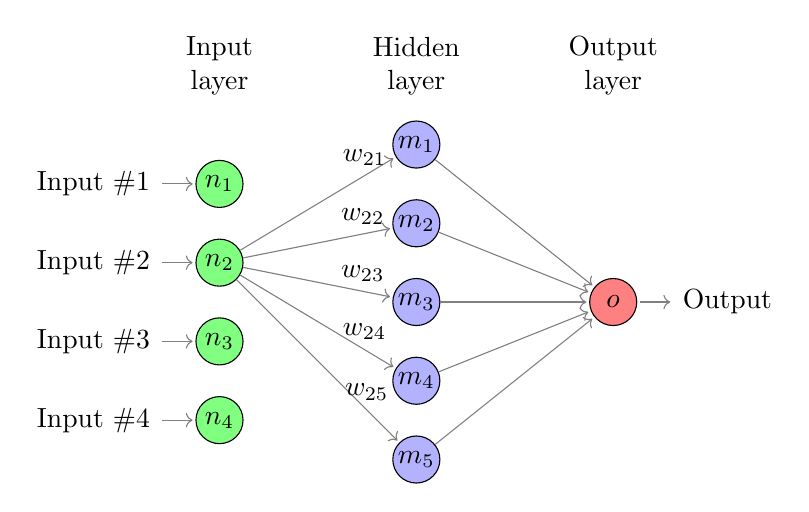
\begin{tikzpicture}[shorten >=1pt,->,draw=black!50, node distance=\layersep]
%https://tex.stackexchange.com/questions/96846/how-to-place-label-in-middle-of-line-above-and-below-with-tikz
    \tikzstyle{every pin edge}=[<-,shorten <=1pt]
    \tikzstyle{neuron}=[circle,fill=black!25,minimum size=17pt,inner sep=0pt, draw=black]
    \tikzstyle{input neuron}=[neuron, fill=green!50];
    \tikzstyle{output neuron}=[neuron, fill=red!50];
    \tikzstyle{hidden neuron}=[neuron, fill=blue!30];
    \tikzstyle{annot} = [text width=4em, text centered]

    % Draw the input layer nodes
    \foreach \name / \y in {1,...,4}
    % This is the same as writing \foreach \name / \y in {1/1,2/2,3/3,4/4}
        \node[input neuron, pin=left:Input \#\y] (I-\name) at (0,-\y) {$n_\y$};

    % Draw the hidden layer nodes
    \foreach \name / \y in {1,...,5}
        \path[yshift=0.5cm]
            node[hidden neuron] (H-\name) at (\layersep,-\y cm) {$m_\y$};

    % Draw the output layer node
    \node[output neuron,pin={[pin edge={->}]right:Output}, right of=H-3] (O) {$o$};

    % Connect every node in the input layer with every node in the
    % hidden layer.
%    \foreach \source in {1,...,4}
%        \foreach \dest in {1,...,5}
%            \draw (I-\source) -- node[below] {$w_ij$} ++ (H-\dest);


%    \foreach \source in {1,...,4}
        \foreach \dest in {1,...,5}
            \draw (I-2) -- node[above, pos=0.8] {$w_{2\dest}$} ++ (H-\dest);

    % Connect every node in the hidden layer with the output layer
    \foreach \source in {1,...,5}
        \path (H-\source) edge (O);

    % Annotate the layers
    \node[annot,above of=H-1, node distance=1cm] (hl) {Hidden layer};
    \node[annot,left of=hl] {Input layer};
    \node[annot,right of=hl] {Output layer};
\end{tikzpicture}
  \end{minipage}
  \vfill
\begin{minipage}[t][0.5\textheight][t]{\textwidth}

\end{minipage}


\end{frame}




\begin{frame}[fragile]{Point Variance of Linear Predictor}

\begin{align*}
\action<+->{ &=&&}
\\
\action<+->{  &=   && }
\end{align*}
\action<+->{The}
\end{frame}



\begin{frame}[fragile]{Correlation}
\begin{itemize}
\item[] \textbf{Serial No.} is basically uncorrelated with anything. \pause
\item[] \textbf{Admit} is highly correlated with \textbf{CGPA}, \textbf{TOEFL Score} and \textbf{GRE Score}\pause
\item[] \textbf{Research} has a lowish correlation with \textbf{Admit}, but also with everything else.  
\end{itemize}
\end{frame}











\begin{frame}[fragile]{Bias, Variance and Parameters}
  \begin{minipage}[t][0.5\textheight][t]{\textwidth}
	\centering
	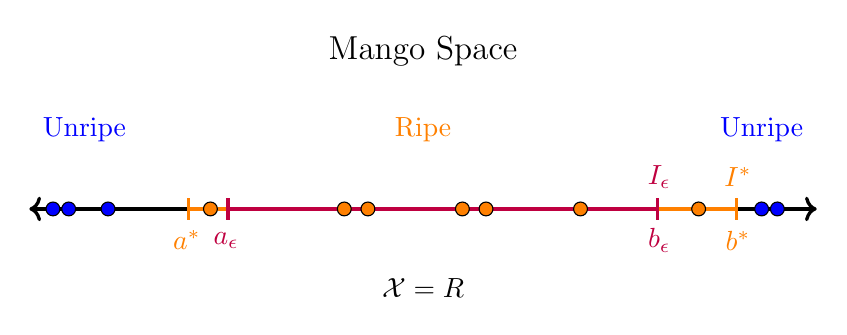
\begin{tikzpicture}
		\draw[<->,very thick] (-5,0) -- (5,0);
		\draw[color = orange, |-|,very thick] (-3,0) -- (4,0);
		\node[color=orange] at (4,.4) {$I^*$};
		\node at (0,2) {\large Mango Space} ;
		\node at (0,-1) {$\mathcal{X} = \mathbb{R}$} ;
		\node [color=blue] at (-4.3,1) {Unripe} ;
		\node [color=blue] at (4.3,1) {Unripe} ;
		\node [color=orange] at (0,1) {Ripe} ;

		\node [color=orange] at (-3,-.4) {$a^*$} ;
		\node [color=orange] at (4,-.4) {$b^*$} ;

		\draw [color=purple, |-|,very thick] (-2.5,0) -- (3,0);
		\node [color=purple] at (3,.4) {$I_\epsilon$} ;
		\node [color=purple] at (-2.5,-.4) {$a_\epsilon$} ;
		\node [color=purple] at (3,-.4) {$b_\epsilon$} ;

%		\draw [color=olive, |-|,very thick] (-3.5,0) -- (2.5,0);
%		\node [color=olive] at (3,.4) {$h_{\mathcal{T}}$} ;



		\node[circle,draw=black, fill=orange, inner sep=0pt,minimum size=5pt] at (2,0) {};
		\node[circle,draw=black, fill=orange, inner sep=0pt,minimum size=5pt] at (-1,0) {};
		\node[circle,draw=black, fill=orange, inner sep=0pt,minimum size=5pt] at (-.7,0) {};
		\node[circle,draw=black, fill=orange, inner sep=0pt,minimum size=5pt] at (.5,0) {};
		\node[circle,draw=black, fill=orange, inner sep=0pt,minimum size=5pt] at (.8,0) {};
		\node[circle,draw=black, fill=orange, inner sep=0pt,minimum size=5pt] at (-2.7,0) {};
		\node[circle,draw=black, fill=orange, inner sep=0pt,minimum size=5pt] at (3.5,0) {};

		\node[circle,draw=black, fill=blue, inner sep=0pt,minimum size=5pt] at (-4.5,0) {};
		\node[circle,draw=black, fill=blue, inner sep=0pt,minimum size=5pt] at (-4,0) {};
		\node[circle,draw=black, fill=blue, inner sep=0pt,minimum size=5pt] at (-4.7,0) {};
		\node[circle,draw=black, fill=blue, inner sep=0pt,minimum size=5pt] at (4.3,0) {};
		\node[circle,draw=black, fill=blue, inner sep=0pt,minimum size=5pt] at (4.5,0) {};
	\end{tikzpicture}
  \end{minipage}
  \vfill
  \begin{minipage}[t][0.5\textheight][t]{\textwidth}
Lets understand this visually.
$$
Err(x_0) = \sigma_\epsilon^2 + [E_\cT[\hat f(x_0)] - f(x_0)]^2 + E_\cT\big[ \hat{f}(x_0) - E_\cT[\hat{f}(x_0)] \big]^2\,.
$$\pause
Consider a data set, 
\end{minipage}
\end{frame}





























